\newpage
\section{Loopy Belief Propagation}

Since exact inference is often computationally expensive, belief propagation (BP) is widely used as an approximate inference algorithm. The procedure starts by constructing a factor graph. We maintain beliefs for all variable nodes and factor nodes, and update them iteratively using a set of message-passing equations. On tree-structured graphs this yields exact marginals, while on graphs with loops, the same procedure (called loopy belief propagation) is only approximate.

The key idea is that if BP converges, it often converges to the correct marginal probabilities (exactly so in trees; approximately so in loopy graphs). However, because this is an iterative approximation algorithm, convergence is not guaranteed in general.

The order of message updates does not strictly matter, as long as all beliefs and messages are eventually updated. In my implementation, I update factor nodes first, then transition nodes, then send messages to variables, update variable beliefs, and finally send messages from variables back to factor and transition nodes. At each iteration, to avoid double counting, the contribution from the previous message that was already incorporated into a belief is divided out before incorporating new messages.

\begin{center}
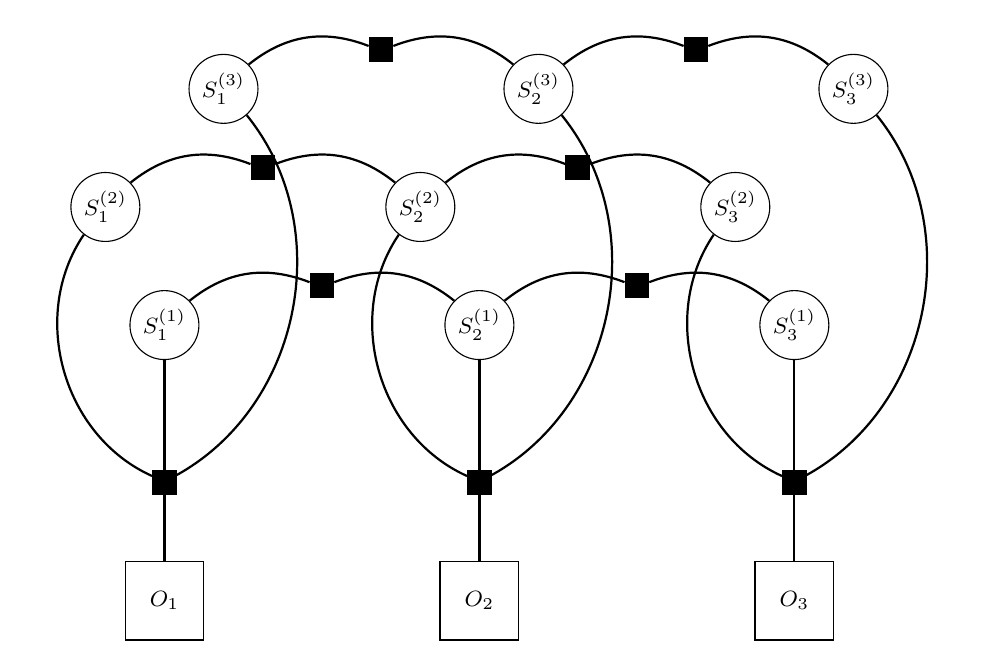
\begin{tikzpicture}[auto,
    var/.style={circle, draw, minimum size=0.8cm, font=\footnotesize, inner sep=2pt},
    factor/.style={rectangle, draw, fill=black, minimum size=0.3cm, font=\footnotesize, inner sep=0pt},
    obs/.style={rectangle, draw, minimum size=1cm, font=\footnotesize, inner sep=2pt},
    every edge/.style={draw, thick}
]

% Hidden state variables for Factor 1 (bottom row)
\node[var] (S1_1) at (0, 4) {$S_1^{(1)}$};
\node[var] (S1_2) at (4, 4) {$S_2^{(1)}$};
\node[var] (S1_3) at (8, 4) {$S_3^{(1)}$};

% Hidden state variables for Factor 2 (middle row, slightly offset)
\node[var] (S2_1) at (-0.75, 5.5) {$S_1^{(2)}$};
\node[var] (S2_2) at (3.25, 5.5) {$S_2^{(2)}$};
\node[var] (S2_3) at (7.25, 5.5) {$S_3^{(2)}$};

% Hidden state variables for Factor 3 (top row, slightly offset)
\node[var] (S3_1) at (0.75, 7) {$S_1^{(3)}$};
\node[var] (S3_2) at (4.75, 7) {$S_2^{(3)}$};
\node[var] (S3_3) at (8.75, 7) {$S_3^{(3)}$};

% Observation variables (below the hidden states)
\node[obs] (O1) at (0, 0.5) {$O_1$};
\node[obs] (O2) at (4, 0.5) {$O_2$};
\node[obs] (O3) at (8,0.5) {$O_3$};

% Factor nodes for transitions in Factor 1
\node[factor] (F1_T1) at (2, 4.5) {};
\node[factor] (F1_T2) at (6, 4.5) {};

% Factor nodes for transitions in Factor 2
\node[factor] (F2_T1) at (1.25, 6) {};
\node[factor] (F2_T2) at (5.25, 6) {};

% Factor nodes for transitions in Factor 3
\node[factor] (F3_T1) at (2.75, 7.5) {};
\node[factor] (F3_T2) at (6.75, 7.5) {};

% Factor nodes for observations
\node[factor] (F_O1) at (0, 2) {};
\node[factor] (F_O2) at (4, 2) {};
\node[factor] (F_O3) at (8, 2) {};

% Edges for Factor 1 transitions
\path (S1_1) edge[bend left=30] (F1_T1);
\path (F1_T1) edge[bend left=30] (S1_2);
\path (S1_2) edge[bend left=30] (F1_T2);
\path (F1_T2) edge[bend left=30] (S1_3);

% Edges for Factor 2 transitions
\path (S2_1) edge[bend left=30] (F2_T1);
\path (F2_T1) edge[bend left=30] (S2_2);
\path (S2_2) edge[bend left=30] (F2_T2);
\path (F2_T2) edge[bend left=30] (S2_3);

% Edges for Factor 3 transitions
\path (S3_1) edge[bend left=30] (F3_T1);
\path (F3_T1) edge[bend left=30] (S3_2);
\path (S3_2) edge[bend left=30] (F3_T2);
\path (F3_T2) edge[bend left=30] (S3_3);

% Edges for observation factors at t=1
\path (S1_1) edge (F_O1);
\path (S2_1) edge[bend right=50] (F_O1);
\path (S3_1) edge[bend left=50] (F_O1);
\path (F_O1) edge (O1);

% Edges for observation factors at t=2
\path (S1_2) edge (F_O2);
\path (S2_2) edge[bend right=50] (F_O2);
\path (S3_2) edge[bend left=50] (F_O2);
\path (F_O2) edge (O2);

% Edges for observation factors at t=3
\path (S1_3) edge (F_O3);
\path (S2_3) edge[bend right=50] (F_O3);
\path (S3_3) edge[bend left=50] (F_O3);
\path (F_O3) edge (O3);

\end{tikzpicture}
\end{center}

Let the number of states be \texttt{K}, number of states be \texttt{N}, number of factors be \texttt{M} and number of observations be \texttt{T}.

\begin{itemize}
    \item The function \texttt{updateFactorNodeBeliefs} has a time complexity of $O(TMK^M)$
    \item The function \texttt{updateTransitionNodeBeliefs} has a time complexity of $O(TMK^2)$
    \item The function \texttt{messageToSendFromFactor} has a time complexity of $O(MK^M)$
    \item The function \texttt{messageToSendFromTransition} has a time complexity of $O(K^2)$
    \item The resulting complexity of function \texttt{sendMessagesToVariables} is $O(TM^2K^M \texttt{+} TMK^2)$
    \item The function \texttt{updateVariableBeliefs} has a time complexity of $O(TMK)$
    \item The function \texttt{sendMessagesToFactorsNodes} has a time complexity of $O(TMK)$
    \item The function \texttt{sendMessagesToTransNodes} has a time complexity of $O(TMK)$
    \item Checking convergence has an order of $O(TMK)$
\end{itemize}
Therefore, the overall time complexity of the algorithm is $O(TM^2K^M \texttt{+} TMK^2)$ assuming O(1) iterations for convergence. 

